%%%%%%%%%%%%%%%%%%%%%%%%%%%%%%%%%%%%%%%%%
% Programming/Coding Assignment
% LaTeX Template
%
% This template has been downloaded from:
% http://www.latextemplates.com
%
% Original author:
% Ted Pavlic (http://www.tedpavlic.com)
%
% Note:
% The \lipsum[#] commands throughout this template generate dummy text
% to fill the template out. These commands should all be removed when 
% writing assignment content.
%
% This template uses a Perl script as an example snippet of code, most other
% languages are also usable. Configure them in the "CODE INCLUSION 
% CONFIGURATION" section.
%
%%%%%%%%%%%%%%%%%%%%%%%%%%%%%%%%%%%%%%%%%

%----------------------------------------------------------------------------------------
%	PACKAGES AND OTHER DOCUMENT CONFIGURATIONS
%----------------------------------------------------------------------------------------

\documentclass{article}

\usepackage{fancyhdr} % Required for custom headers
\usepackage{lastpage} % Required to determine the last page for the footer
\usepackage{extramarks} % Required for headers and footers
\usepackage[usenames,dvipsnames]{color} % Required for custom colors
\usepackage{graphicx} % Required to insert images
\usepackage{listings} % Required for insertion of code
\usepackage{courier} % Required for the courier font
\usepackage{lipsum} % Used for inserting dummy 'Lorem ipsum' text into the template

\usepackage{paralist}
% Margins
\topmargin=-0.45in
\evensidemargin=0in
\oddsidemargin=0in
\textwidth=6.5in
\textheight=9.0in
\headsep=0.25in

\linespread{1.1} % Line spacing

% Set up the header and footer
\pagestyle{fancy}
\lhead{\hmwkAuthorNameShort} % Top left header
\chead{\hmwkClass:\ \hmwkTitle} % Top center head
\rhead{} % Top right header
\lfoot{} % Bottom left footer
\cfoot{} % Bottom center footer
\rfoot{Page\ \thepage\ of\ \protect\pageref{LastPage}} % Bottom right footer
\renewcommand\headrulewidth{0.4pt} % Size of the header rule
\renewcommand\footrulewidth{0.4pt} % Size of the footer rule

%\setlength\parindent{0pt} % Removes all indentation from paragraphs

%----------------------------------------------------------------------------------------
%	CODE INCLUSION CONFIGURATION
%----------------------------------------------------------------------------------------
\definecolor{mygreen}{rgb}{0,0.6,0}
\definecolor{mygray}{rgb}{0.5,0.5,0.5} 
\definecolor{mymauve}{rgb}{0.58,0,0.82}

\lstset{ %
  backgroundcolor=\color{white},   % choose the background color; you must add \usepackage{color} or \usepackage{xcolor}
  basicstyle=\footnotesize,        % the size of the fonts that are used for the code
  breakatwhitespace=false,         % sets if automatic breaks should only happen at whitespace
  breaklines=true,                 % sets automatic line breaking
  captionpos=b,                    % sets the caption-position to bottom
  commentstyle=\color{mygreen},    % comment style
  deletekeywords={...},            % if you want to delete keywords from the given language
  escapeinside={\%*}{*)},          % if you want to add LaTeX within your code
  extendedchars=true,              % lets you use non-ASCII characters; for 8-bits encodings only, does not work with UTF-8
  frame=single,                    % adds a frame around the code
  keepspaces=true,                 % keeps spaces in text, useful for keeping indentation of code (possibly needs columns=flexible)
  keywordstyle=\color{blue},       % keyword style
  language=Octave,                 % the language of the code
  morekeywords={*,...},            % if you want to add more keywords to the set
  numbers=left,                    % where to put the line-numbers; possible values are (none, left, right)
  numbersep=5pt,                   % how far the line-numbers are from the code
  numberstyle=\tiny\color{mygray}, % the style that is used for the line-numbers
  rulecolor=\color{black},         % if not set, the frame-color may be changed on line-breaks within not-black text (e.g. comments (green here))
  showspaces=false,                % show spaces everywhere adding particular underscores; it overrides 'showstringspaces'
  showstringspaces=false,          % underline spaces within strings only
  showtabs=false,                  % show tabs within strings adding particular underscores
  stepnumber=2,                    % the step between two line-numbers. If it's 1, each line will be numbered
  stringstyle=\color{mymauve},     % string literal style
  tabsize=2,                       % sets default tabsize to 2 spaces
  title=\lstname                   % show the filename of files included with \lstinputlisting; also try caption instead of title
}


\newcommand{\includecode}[3]{\lstinputlisting[caption=#2,captionpos=t,language=Java,label=#3]{code/#1}}


%----------------------------------------------------------------------------------------
%	NAME AND CLASS SECTION
%----------------------------------------------------------------------------------------

\newcommand{\hmwkTitle}{Milestone\ \#1} % Assignment title
\newcommand{\hmwkDueDate}{\today} % Due date
\newcommand{\hmwkClass}{COMP\ 512} % Course/class
\newcommand{\hmwkAuthorName}{Jonah Caplan, Haitong Yang} % Your name
\newcommand{\hmwkAuthorNameShort}{Caplan, Yang} % Your name

%----------------------------------------------------------------------------------------
%	TITLE PAGE
%----------------------------------------------------------------------------------------

\title{
\vspace{2in}
\textmd{\textbf{\hmwkClass:\ \hmwkTitle}}\\
\vspace{3in}
}

\author{\textbf{\hmwkAuthorName}}
\date{} % Insert date here if you want it to appear below your name



%----------------------------------------------------------------------------------------

\begin{document}

\maketitle
\thispagestyle{empty}
\newpage
\setcounter{page}{1}

%------------------------------------------------------------------------------------
\section{Deliverables}
The following deliverables are required for the first project milestone:
\begin{description}
\item[Distributed web services] \hfill \\ Distribute a pre-existing
server/client system built on web services.
\item[TCP Implementation] \hfill \\ Implement the same distributed system using
TCP instead of web services.
\end{description}


\section{Distributed web services}

The distributed system consists of three components: the end-user client, the middleware (MW), and the resource manager (RM) servers. 
We chose to have four RMs: one for each type of reservation item as well as one for customers. 
The middleware consists of a client and a server both of which are modified versions of the original code provided. 
The main functionality that differentiates the MW from the RMs is the booking of itineraries which requires coordination between the MW and each RM. 


This section will briefly describe the changes made to the client and RMs and then discuss the middleware design. We assume the reader is familiar with the original source code.

\subsection{Client modifications}
No modifications were required for the Client implementation. 
For convenience, the parsing of commands was separated from the main run loop in order to facilitate test writing by providing a code-based interface to enter commands.
	
	
\subsection{RM server modifications}
The server required several modifications to support the middleware. 
The original RM implementation assumed that customer information was located in the same hash table as the services. 
The reservation of items consisted of two main steps: check that the item was available and reserve it, then update the customer data structure so the reserved item is on their bill. 
In order to allow the middleware to coordinate this process among the RMs, it was necessary to seperate the reservation of items and the updating of customer data into separate methods and to expose these methods to the ResourceManager interface. 
It was also necessary to allow the MW to cancel a reservation (details in the section on MW). 
Methods were added to the interface to allow explicit updating of the customer reservations and cancelling reservations on specific items. 
    	
\subsection{Middleware implementation}

The middleware implementation is fairly straight-forward. 
It consists of a server that implements the ResourceManager interface. Upon a call from a client, the MW methods create a new client object to pass the request to the appropriate RM server.

The main difficulty in the MW design is to safely handle the itinerary requests which consist of one or several flights as well as a room and car reservation. 
The algorithm for reserving an itinerary is shown in Figure~\ref{f:res-itin}. The MW attempts to successively reserve each item in the itinerary. The itinerary is cancelled if any of the items cannot be reserved. In this case the RMs must be notified for each item that was successfully reserved. 

A similar approach was used for deleting customers. In this case, the customer's bill was retrieved from the client RM and each item was cancelled.

\begin{figure}
\centering
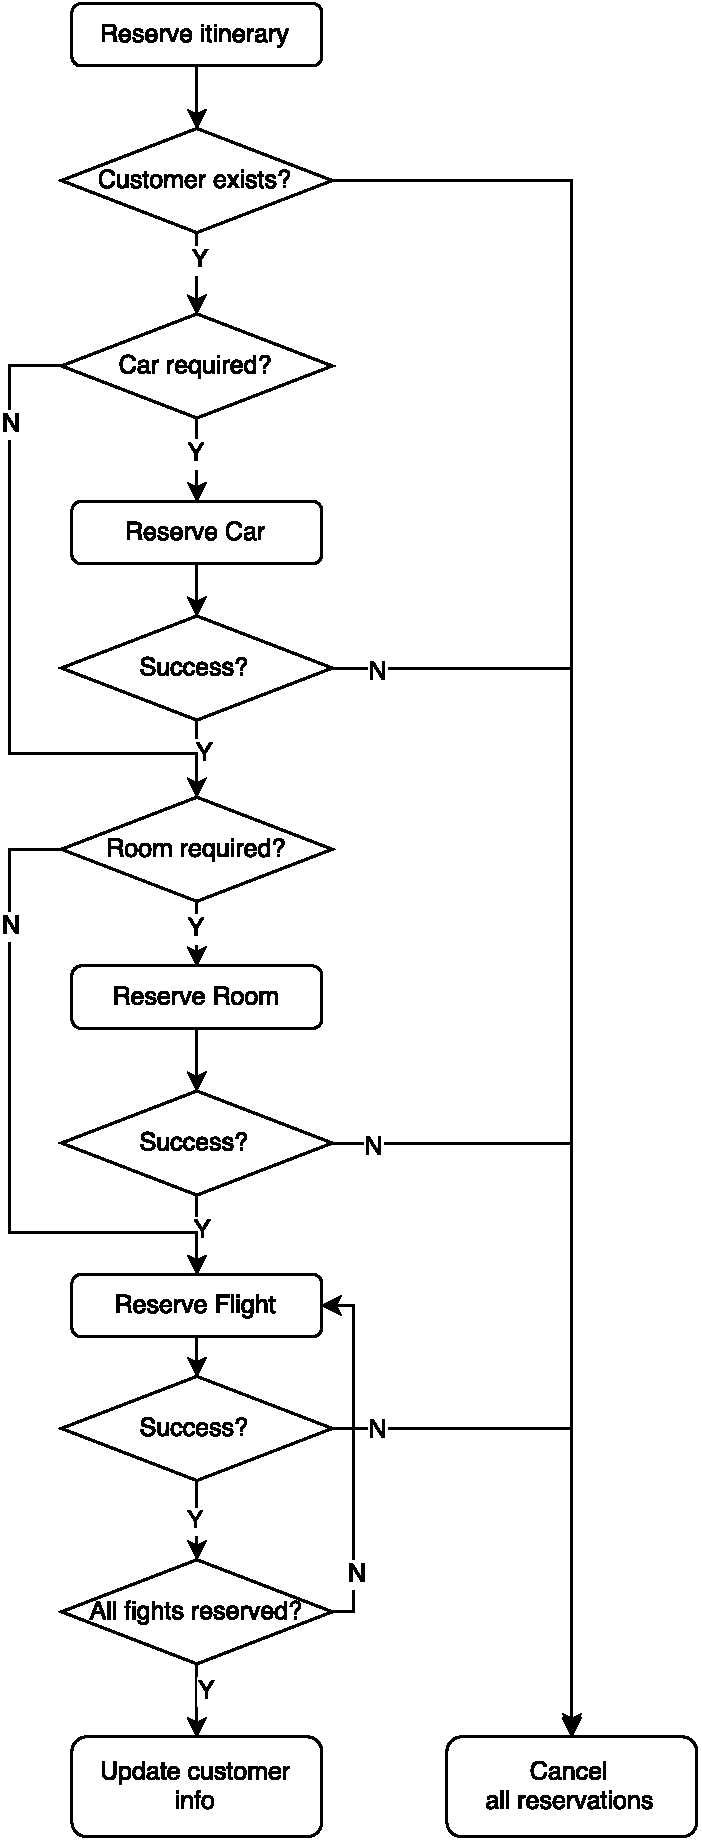
\includegraphics[scale=0.6]{figures/res-itin}
\caption{Algorithm for reserving itinerary.}
\label{f:res-itin}
\end{figure}

\subsection{Synchronization issues}

The code provided ensured that only one thread can have read or write access to the RMs hash table at a time. 
This is not sufficient as the following example will illustrate. 
Consider the code in Listing~\ref{l:ex}. 
First, the object \texttt{curObj} must be retrieved from the hash table and we know that this is itself a safe retrieval and \texttt{curObj} may not be corrupted. 
At line 6 there is a check to see if \texttt{curObj} is null. 
This check is potentially unsafe because it could be that \texttt{curObj} is not null at line 6 but is null at line 11. 
It may be tempting to synchronize on \texttt{curObj} itself, but this is potentially a null pointer exception if the synchronization occurs before the check at line 5. 
Postponing the synchronization block until line 10 results in the exact same problem as before. 
It is necessary to synchronize all accesses to objects from the moment their reference is retrieved until the actions that must be taken with them are completed. 
The updated code is shown in Listing~\ref{l:ex-sync}.

There is another issue regarding the deletion of clients. It is possible that a flight could be deleted after the MW retrieves the customer data but before the flights can be cancelled. It does not seem like an adequate solution to force a synchronized block at the middleware level. This may be less of a synchronization issue and more of a domain specific issue. An argument could be made that this type of error must be caught by the middleware and appropriate actions (e.g. cancellation or refund) should be initiated. Note that this problem does not create a runtime error but we do feel that some extra actions should be taken by the middleware in case the cancellation of a reservation fails.

\includecode{example.java}{This code has several potential synchronization issues.}{l:ex}

\includecode{example-sync.java}{Almost the entire method body must be synchronized to prevent potential null pointer exceptions.}{l:ex-sync}

\section{TCP Implementation} 

Our design goals for the TCP based system were to reuse as much of the original code as possible and to simplify the communication protocol. 
We wanted to avoid spending time debugging the passing of messages between processes and instead focus on the actions taken by each process based on the information contained in the message. 

\section{Communication protocol}
Very little information needs to flow between processes and code already existed to manually parse command line entries from the client. 
It made sense to have the client send unparsed commands directly over TCP and move the pre-existing code for parsing commands to the RMs. 
Setting up the command parsing on the RM was very simple because the client code was already designed to interface with the \texttt{ResourceManagerImpl} class.  
The middleware would then parse the first argument in the command and forward it to the correct RM. 
The RM then fully parses the command and updates its data structures accordingly. 
In the case of reserving an itinerary, the MW needed to parse the entire command and build new commands to make reservations with each RM. 
The RMs always return a string representing the original integer or boolean return types. 

The possible downside of transmitting information in this manner is that manually constructing and parsing strings may prove cumbersome and error prone if large data types were required. 
Packing information into objects and relying on java to serialize their represention would be easier to manage if the data passing between processes was more complex. 
However, we think our current implementation is fairly lightweight and effective given that parsing code was already provided and the small message sizes. 
If we had more time or if this were a real (i.e. not class) and possibly agile design project, it might still have made sense to start with this design as a transitional step towards a more robust implementation using objects as we don't want to change too much of the implementation in a single iteration. 
 



\section{Thread management in middleware and resource managers}

A new thread must be created in the MW or RM when a client connects to the MW or the MW connects to the RM for a specific client, respectively. This allows as much work to be done concurrently per client as possible despite the fact that some RM methods must be synchronized. The basic flow is shown in Figure~\ref{f:threads}. Both clients must initially pass through the main thread when initiating communication. The main MW thread then creates a dedicated thread to deal with that client. The same process occurs between the MW and the RM. The client communicates directly with the dedicated thread when it makes future requests.

\begin{figure}
\centering
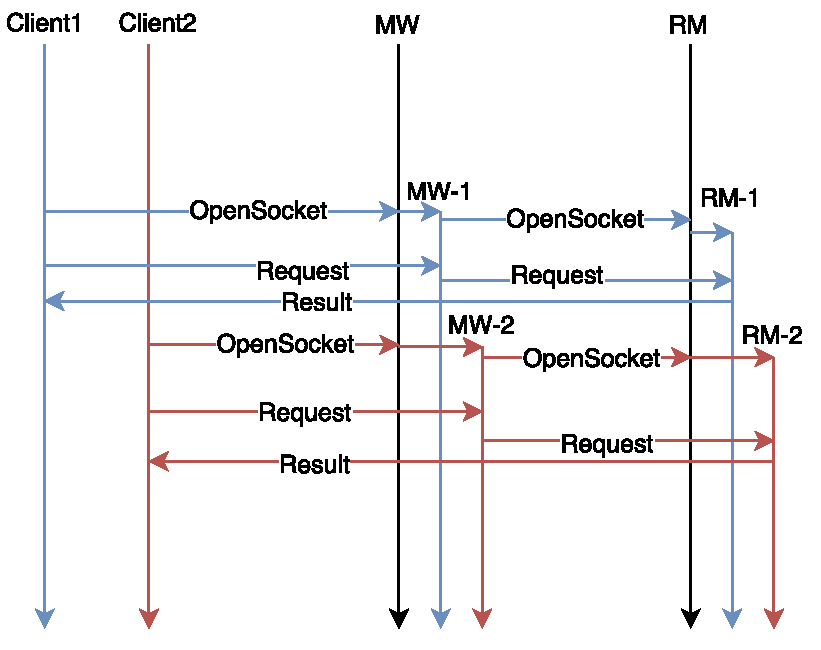
\includegraphics[scale=1]{figures/threads.pdf}
\caption{Two clients communicate with RM through the MW at same time.}
\label{f:threads}
\end{figure} 


\end{document}